% Options for packages loaded elsewhere
\PassOptionsToPackage{unicode}{hyperref}
\PassOptionsToPackage{hyphens}{url}
%
\documentclass[
  10pt,
]{article}
\usepackage{amsmath,amssymb}
\usepackage{iftex}
\ifPDFTeX
  \usepackage[T1]{fontenc}
  \usepackage[utf8]{inputenc}
  \usepackage{textcomp} % provide euro and other symbols
\else % if luatex or xetex
  \usepackage{unicode-math} % this also loads fontspec
  \defaultfontfeatures{Scale=MatchLowercase}
  \defaultfontfeatures[\rmfamily]{Ligatures=TeX,Scale=1}
\fi
\usepackage{lmodern}
\ifPDFTeX\else
  % xetex/luatex font selection
\fi
% Use upquote if available, for straight quotes in verbatim environments
\IfFileExists{upquote.sty}{\usepackage{upquote}}{}
\IfFileExists{microtype.sty}{% use microtype if available
  \usepackage[]{microtype}
  \UseMicrotypeSet[protrusion]{basicmath} % disable protrusion for tt fonts
}{}
\makeatletter
\@ifundefined{KOMAClassName}{% if non-KOMA class
  \IfFileExists{parskip.sty}{%
    \usepackage{parskip}
  }{% else
    \setlength{\parindent}{0pt}
    \setlength{\parskip}{6pt plus 2pt minus 1pt}}
}{% if KOMA class
  \KOMAoptions{parskip=half}}
\makeatother
\usepackage{xcolor}
\usepackage[margin=1in]{geometry}
\usepackage{longtable,booktabs,array}
\usepackage{multirow}
\usepackage{calc} % for calculating minipage widths
% Correct order of tables after \paragraph or \subparagraph
\usepackage{etoolbox}
\makeatletter
\patchcmd\longtable{\par}{\if@noskipsec\mbox{}\fi\par}{}{}
\makeatother
% Allow footnotes in longtable head/foot
\IfFileExists{footnotehyper.sty}{\usepackage{footnotehyper}}{\usepackage{footnote}}
\makesavenoteenv{longtable}
\usepackage{graphicx}
\makeatletter
\def\maxwidth{\ifdim\Gin@nat@width>\linewidth\linewidth\else\Gin@nat@width\fi}
\def\maxheight{\ifdim\Gin@nat@height>\textheight\textheight\else\Gin@nat@height\fi}
\makeatother
% Scale images if necessary, so that they will not overflow the page
% margins by default, and it is still possible to overwrite the defaults
% using explicit options in \includegraphics[width, height, ...]{}
\setkeys{Gin}{width=\maxwidth,height=\maxheight,keepaspectratio}
% Set default figure placement to htbp
\makeatletter
\def\fps@figure{htbp}
\makeatother
\ifLuaTeX
  \usepackage{luacolor}
  \usepackage[soul]{lua-ul}
\else
  \usepackage{soul}
\fi
\setlength{\emergencystretch}{3em} % prevent overfull lines
\providecommand{\tightlist}{%
  \setlength{\itemsep}{0pt}\setlength{\parskip}{0pt}}
\setcounter{secnumdepth}{-\maxdimen} % remove section numbering
\ifLuaTeX
  \usepackage{selnolig}  % disable illegal ligatures
\fi
\ifPDFTeX
  \TeXXeTstate=1
  \newcommand{\RL}[1]{\beginR #1\endR}
  \newcommand{\LR}[1]{\beginL #1\endL}
  \newenvironment{RTL}{\beginR}{\endR}
  \newenvironment{LTR}{\beginL}{\endL}
\fi
\usepackage{bookmark}
\IfFileExists{xurl.sty}{\usepackage{xurl}}{} % add URL line breaks if available
\urlstyle{same}
\hypersetup{
  hidelinks,
  pdfcreator={LaTeX via pandoc}}

\author{}
\date{}

\providecommand{\RL}[1]{#1}
\begin{document}

\begin{longtable}[]{@{}
  >{\raggedright\arraybackslash}p{(\columnwidth - 10\tabcolsep) * \real{0.2399}}
  >{\raggedright\arraybackslash}p{(\columnwidth - 10\tabcolsep) * \real{0.1361}}
  >{\raggedright\arraybackslash}p{(\columnwidth - 10\tabcolsep) * \real{0.1528}}
  >{\raggedright\arraybackslash}p{(\columnwidth - 10\tabcolsep) * \real{0.1529}}
  >{\raggedright\arraybackslash}p{(\columnwidth - 10\tabcolsep) * \real{0.1805}}
  >{\raggedright\arraybackslash}p{(\columnwidth - 10\tabcolsep) * \real{0.1377}}@{}}
\toprule\noalign{}
\begin{minipage}[b]{\linewidth}\raggedright
Methods
\end{minipage} & \begin{minipage}[b]{\linewidth}\raggedright
Year
\end{minipage} & \begin{minipage}[b]{\linewidth}\raggedright
Parameters
\end{minipage} & \begin{minipage}[b]{\linewidth}\raggedright
Dice
\end{minipage} & \begin{minipage}[b]{\linewidth}\raggedright
iou
\end{minipage} & \begin{minipage}[b]{\linewidth}\raggedright
Input size
\end{minipage} \\
\midrule\noalign{}
\endhead
\bottomrule\noalign{}
\endlastfoot
TransNetR (4) & 2023 & 27.27 & 87.06 & 80.16 & ? \\
SegMed-Net \RL{}(8) & \RL{2026} & 59.9 & 90.8 & 83.70 & 352*352 \\
PVT-Cascade (3) & 2023 & 35.2 & 91.1 & 86.3 & 352*352 \\
MegaNet (2) & 2024 & 44.1 & 91.3 & 86.3 & 352*352 \\
Fu-TransHNet (5) & 2023 & ? & 91.6 & 86.6 & 352*352 \\
LiteBoundD (1) & 2026 & 32.8 & 91.9 & 84.1 & 352*352 \\
AAPCNet (7) & 2025 & 38.2 & 92.10 & 86.9 & 256*256 \\
DVFIP-Net & 2026 & \RL{45.62} & \RL{92.20} & \RL{87.40} & 352*352 \\
SAM2-FNet & 2026 & \RL{27.2} & \RL{92.40} & 87.40 & 352*352 \\
MLB-Net & 2026 & 87.7 & 92.60 & 87.80 & 352*352 \\
MSPN & 2026 & 28.56 & 92.70 & 87.90 & 352*352 \\
HCA-Net & 2026 & 89.70 & 93.60 & 89.7 & 352*352 \\
Ours & 2026 & 38.5 & 93.89 & 88.66 & 352*352 \\
PolyMamba-Net~(6) & 2026 & 25.3 & 94.2 & 89.1 & 352*352 \\
\end{longtable}

\begin{enumerate}
\def\labelenumi{\arabic{enumi}.}
\item
  Sharpening Lightweight Models for Generalized Polyp Segmentation: A
  Boundary Guided Distillation from Foundation Models
\item
  ``Meganet: Multi-scale edge-guided attention network for weak boundary
  polyp segmentation
\item
  ``Medical image segmentation via cascaded attention decoding
\item
  TransNetR: Transformer-based Residual Network for Polyp Segmentation
  with Multi-Center Out-of-Distribution Testin
\item
  Cooperation Learning Enhanced Colonic Polyp Segmentation Based on
  TransformerCNN Fusion
\item
  PolyMamba-Net: a lightweight and boundary-aware network for real-time
  polyp segmentation in colonoscopy
\item
  Attention-Guided Asymmetric Multiscale Polyp Segmentation Network
\item
  SegMed-Net: a domain-aware dual encoder-decoder network with dense
  feature fusion for enhanced medical image segmentation
\end{enumerate}

\textbf{Boundary-Frequency Injection Module:}

\begin{itemize}
\item
  Decomposing frequency components~

  \begin{itemize}
  \item
    Frequency Feature Decomposer (FFD)
  \item
    Spilt skip features into high-frequency and low-frequency using 2D
    FFT

    \begin{itemize}
    \item
      High-frequency -\textgreater{} Boundaries, edges
    \item
      Low-frequency -\textgreater{} semantic content
    \end{itemize}
  \end{itemize}
\item
  Using boundary information for better feature guidance

  \begin{itemize}
  \item
    Boundary-guided Squeeze-Excitation Injection (BSEI)
  \item
    Uses Sobel operators to detect boundaries in skip features
  \item
    Creates spatial attention maps from boundary information
  \item
    Uses cross-attention between decoder features and boundary-weighted
    encoder features
  \end{itemize}
\item
  Adaptively fusing these different feature representations

  \begin{itemize}
  \item
    Multi-scale Frequency Adaptive Fusion (MFAF)
  \item
    Learns soft weights to combine high-frequency, low-frequency, and
    boundary-enhanced features
  \item
    Uses channel-wise gating to decide the importance of each component
  \end{itemize}
\end{itemize}

\textbf{Purpose:}

The BFIM replaces standard skip connections to:

\begin{itemize}
\item
  \textbf{Better preserve boundary information}~during up-sampling
\item
  \textbf{Adaptively emphasize}~important frequency components
\item
  \textbf{Improve segmentation accuracy}~especially for object
  boundaries
\item
  \textbf{Provide learnable fusion}~instead of simple concatenation
\end{itemize}

\begin{longtable}[]{@{}
  >{\raggedright\arraybackslash}p{(\columnwidth - 22\tabcolsep) * \real{0.0930}}
  >{\raggedright\arraybackslash}p{(\columnwidth - 22\tabcolsep) * \real{0.1137}}
  >{\raggedright\arraybackslash}p{(\columnwidth - 22\tabcolsep) * \real{0.0804}}
  >{\raggedright\arraybackslash}p{(\columnwidth - 22\tabcolsep) * \real{0.0822}}
  >{\raggedright\arraybackslash}p{(\columnwidth - 22\tabcolsep) * \real{0.0794}}
  >{\raggedright\arraybackslash}p{(\columnwidth - 22\tabcolsep) * \real{0.0785}}
  >{\raggedright\arraybackslash}p{(\columnwidth - 22\tabcolsep) * \real{0.0783}}
  >{\raggedright\arraybackslash}p{(\columnwidth - 22\tabcolsep) * \real{0.0794}}
  >{\raggedright\arraybackslash}p{(\columnwidth - 22\tabcolsep) * \real{0.0777}}
  >{\raggedright\arraybackslash}p{(\columnwidth - 22\tabcolsep) * \real{0.0767}}
  >{\raggedright\arraybackslash}p{(\columnwidth - 22\tabcolsep) * \real{0.0767}}
  >{\raggedright\arraybackslash}p{(\columnwidth - 22\tabcolsep) * \real{0.0840}}@{}}
\toprule\noalign{}
\multirow{3}{=}{\begin{minipage}[b]{\linewidth}\raggedright
Models
\end{minipage}} &
\multicolumn{4}{>{\raggedright\arraybackslash}p{(\columnwidth - 22\tabcolsep) * \real{0.3557} + 6\tabcolsep}}{%
\begin{minipage}[b]{\linewidth}\raggedright
\textbf{Seen}
\end{minipage}} &
\multicolumn{6}{>{\raggedright\arraybackslash}p{(\columnwidth - 22\tabcolsep) * \real{0.4674} + 10\tabcolsep}}{%
\begin{minipage}[b]{\linewidth}\raggedright
\textbf{Unseen}
\end{minipage}} & \begin{minipage}[b]{\linewidth}\raggedright
\textbf{Epoch}
\end{minipage} \\
&
\multicolumn{2}{>{\raggedright\arraybackslash}p{(\columnwidth - 22\tabcolsep) * \real{0.1941} + 2\tabcolsep}}{%
\begin{minipage}[b]{\linewidth}\raggedright
\textbf{Kvasir-Seg}
\end{minipage}} &
\multicolumn{2}{>{\raggedright\arraybackslash}p{(\columnwidth - 22\tabcolsep) * \real{0.1616} + 2\tabcolsep}}{%
\begin{minipage}[b]{\linewidth}\raggedright
\textbf{ClinicDB}
\end{minipage}} &
\multicolumn{2}{>{\raggedright\arraybackslash}p{(\columnwidth - 22\tabcolsep) * \real{0.1568} + 2\tabcolsep}}{%
\begin{minipage}[b]{\linewidth}\raggedright
\textbf{CVC-300}
\end{minipage}} &
\multicolumn{2}{>{\raggedright\arraybackslash}p{(\columnwidth - 22\tabcolsep) * \real{0.1571} + 2\tabcolsep}}{%
\begin{minipage}[b]{\linewidth}\raggedright
\textbf{ColonDB}
\end{minipage}} &
\multicolumn{2}{>{\raggedright\arraybackslash}p{(\columnwidth - 22\tabcolsep) * \real{0.1535} + 2\tabcolsep}}{%
\begin{minipage}[b]{\linewidth}\raggedright
\textbf{ETIS}
\end{minipage}} & \begin{minipage}[b]{\linewidth}\raggedright
\end{minipage} \\
& \begin{minipage}[b]{\linewidth}\raggedright
Dice
\end{minipage} & \begin{minipage}[b]{\linewidth}\raggedright
iou
\end{minipage} & \begin{minipage}[b]{\linewidth}\raggedright
Dice
\end{minipage} & \begin{minipage}[b]{\linewidth}\raggedright
iou
\end{minipage} & \begin{minipage}[b]{\linewidth}\raggedright
Dice
\end{minipage} & \begin{minipage}[b]{\linewidth}\raggedright
iou
\end{minipage} & \begin{minipage}[b]{\linewidth}\raggedright
Dice
\end{minipage} & \begin{minipage}[b]{\linewidth}\raggedright
iou
\end{minipage} & \begin{minipage}[b]{\linewidth}\raggedright
Dice
\end{minipage} & \begin{minipage}[b]{\linewidth}\raggedright
iou
\end{minipage} & \begin{minipage}[b]{\linewidth}\raggedright
\end{minipage} \\
\midrule\noalign{}
\endhead
\bottomrule\noalign{}
\endlastfoot
HCA-Net & 93.6 & 89.7 & 95.6 & 90.9 & 91.2 & 87.3 & 83.4 & 76.9 & 83.3 &
78.9 & \\
Ours & 92.40 & 86.08 & 95.19 & 90.84 & \textbf{91.49} & 84.32 & 81.26 &
70.44 & \textbf{87.39} & \textbf{77.61} & \textbf{1370} \\
Ours-2 & 92.58 & 86.41 & 95.31 & 91.04 & & & 81.45 & 70.95 & & &
\textbf{1405} \\
& 92.03 & & 95.27 & 90.97 & & & 83.34 & 73.75 & & & \\
\end{longtable}

\begin{longtable}[]{@{}
  >{\raggedright\arraybackslash}p{(\columnwidth - 22\tabcolsep) * \real{0.0943}}
  >{\raggedright\arraybackslash}p{(\columnwidth - 22\tabcolsep) * \real{0.0847}}
  >{\raggedright\arraybackslash}p{(\columnwidth - 22\tabcolsep) * \real{0.0843}}
  >{\raggedright\arraybackslash}p{(\columnwidth - 22\tabcolsep) * \real{0.0875}}
  >{\raggedright\arraybackslash}p{(\columnwidth - 22\tabcolsep) * \real{0.0829}}
  >{\raggedright\arraybackslash}p{(\columnwidth - 22\tabcolsep) * \real{0.0813}}
  >{\raggedright\arraybackslash}p{(\columnwidth - 22\tabcolsep) * \real{0.0811}}
  >{\raggedright\arraybackslash}p{(\columnwidth - 22\tabcolsep) * \real{0.0829}}
  >{\raggedright\arraybackslash}p{(\columnwidth - 22\tabcolsep) * \real{0.0801}}
  >{\raggedright\arraybackslash}p{(\columnwidth - 22\tabcolsep) * \real{0.0784}}
  >{\raggedright\arraybackslash}p{(\columnwidth - 22\tabcolsep) * \real{0.0784}}
  >{\raggedright\arraybackslash}p{(\columnwidth - 22\tabcolsep) * \real{0.0842}}@{}}
\toprule\noalign{}
\multirow{3}{=}{\begin{minipage}[b]{\linewidth}\raggedright
Models
\end{minipage}} &
\multicolumn{4}{>{\raggedright\arraybackslash}p{(\columnwidth - 22\tabcolsep) * \real{0.3395} + 6\tabcolsep}}{%
\begin{minipage}[b]{\linewidth}\raggedright
\textbf{Seen}
\end{minipage}} &
\multicolumn{6}{>{\raggedright\arraybackslash}p{(\columnwidth - 22\tabcolsep) * \real{0.4821} + 10\tabcolsep}}{%
\begin{minipage}[b]{\linewidth}\raggedright
\textbf{Unseen}
\end{minipage}} & \begin{minipage}[b]{\linewidth}\raggedright
\textbf{Epoch}
\end{minipage} \\
&
\multicolumn{2}{>{\raggedright\arraybackslash}p{(\columnwidth - 22\tabcolsep) * \real{0.1690} + 2\tabcolsep}}{%
\begin{minipage}[b]{\linewidth}\raggedright
\textbf{Kvasir-Seg}
\end{minipage}} &
\multicolumn{2}{>{\raggedright\arraybackslash}p{(\columnwidth - 22\tabcolsep) * \real{0.1704} + 2\tabcolsep}}{%
\begin{minipage}[b]{\linewidth}\raggedright
\textbf{ClinicDB}
\end{minipage}} &
\multicolumn{2}{>{\raggedright\arraybackslash}p{(\columnwidth - 22\tabcolsep) * \real{0.1624} + 2\tabcolsep}}{%
\begin{minipage}[b]{\linewidth}\raggedright
\textbf{CVC-300}
\end{minipage}} &
\multicolumn{2}{>{\raggedright\arraybackslash}p{(\columnwidth - 22\tabcolsep) * \real{0.1629} + 2\tabcolsep}}{%
\begin{minipage}[b]{\linewidth}\raggedright
\textbf{ColonDB}
\end{minipage}} &
\multicolumn{2}{>{\raggedright\arraybackslash}p{(\columnwidth - 22\tabcolsep) * \real{0.1568} + 2\tabcolsep}}{%
\begin{minipage}[b]{\linewidth}\raggedright
\textbf{ETIS}
\end{minipage}} & \begin{minipage}[b]{\linewidth}\raggedright
\end{minipage} \\
& \begin{minipage}[b]{\linewidth}\raggedright
Dice
\end{minipage} & \begin{minipage}[b]{\linewidth}\raggedright
iou
\end{minipage} & \begin{minipage}[b]{\linewidth}\raggedright
Dice
\end{minipage} & \begin{minipage}[b]{\linewidth}\raggedright
iou
\end{minipage} & \begin{minipage}[b]{\linewidth}\raggedright
Dice
\end{minipage} & \begin{minipage}[b]{\linewidth}\raggedright
iou
\end{minipage} & \begin{minipage}[b]{\linewidth}\raggedright
Dice
\end{minipage} & \begin{minipage}[b]{\linewidth}\raggedright
iou
\end{minipage} & \begin{minipage}[b]{\linewidth}\raggedright
Dice
\end{minipage} & \begin{minipage}[b]{\linewidth}\raggedright
iou
\end{minipage} & \begin{minipage}[b]{\linewidth}\raggedright
\end{minipage} \\
\midrule\noalign{}
\endhead
\bottomrule\noalign{}
\endlastfoot
HCA-Net & 93.6 & 89.7 & 95.6 & 90.9 & 91.2 & 87.3 & 83.4 & 76.9 & 83.3 &
78.9 & \\
& 93.49 & 87.77 & 95.31 & 91.04 & \textbf{91.61} & 84.52 & 83.34 & 73.75
& \textbf{88.69} & \textbf{79.67} & \\
Our & \hl{93.49} & \hl{87.77} & 94.92 & 90.33 & \textbf{90.33} & 82.52 &
79.72 & 69.16 & \textbf{\hl{88.69}} & \textbf{\hl{79.67}} &
\textbf{100} \\
Ours & 92.58 & 86.41 & \hl{95.31} & \hl{91.04} & \textbf{91.49} & 84.32
& \hl{83.34} & \hl{73.75} & \textbf{87.39} & \textbf{77.61} &
\textbf{1370} \\
Ours-93.04 & \RL{92.30} & & & & \textbf{\RL{91.25}} & \RL{83.91} & & &
\textbf{84.96} & \textbf{73.85} & \\
Ours-93.66 & 92.75 & 86.48 & 95.20 & 90.83 & \textbf{\hl{91.61}} &
\hl{84.52} & 82.81 & 72.96 & \textbf{85.39} & \textbf{74.50} &
\textbf{2836} \\
\end{longtable}

\section{Introduction}

Colorectal polyps are abnormal tissue growths that can develop into malignant lesions if they are not detected and removed at an early stage. Colonoscopy is widely used for the examination of the lower gastrointestinal tract and enables clinicians to identify and remove suspicious lesions. Nevertheless, visual inspection remains challenging because polyp appearance varies considerably across patients and imaging conditions. Variations in lesion size, morphology, texture, contrast, and location, together with specular reflections, motion blur, intestinal folds, bubbles, and other visual artifacts, can complicate accurate delineation of polyp regions. Automated polyp segmentation therefore remains an important problem in computer-aided colonoscopy, where reliable pixel-level localization may assist subsequent analysis and clinical decision support.

Accurate polyp segmentation requires a model to simultaneously capture high-level semantic information and preserve sufficiently detailed spatial representations. U-shaped encoder--decoder architectures are well suited to this task because they combine progressively abstract encoder features with higher-resolution representations through skip connections. U-Net established this general design, while subsequent architectures such as UNet++ further demonstrated the importance of multi-level feature interaction and hierarchical decoding \cite{unet,unetpp}. However, repeated downsampling reduces spatial resolution, and fixed decoder operations may not always provide sufficient flexibility for lesions that vary considerably in scale and visual frequency content.

Recent transformer-based and hybrid architectures have improved long-range dependency modeling in medical image segmentation. TransUNet combines convolutional representations with transformer encoding, while Polyp-PVT applies hierarchical transformer features and cross-level aggregation to polyp segmentation \cite{transunet,polyppvt}. These approaches demonstrate the importance of broad contextual modeling, but they can introduce additional architectural complexity. Modern convolutional networks such as ConvNeXt provide an alternative by retaining the efficiency and spatial inductive bias of convolution while incorporating design principles that improve representation capacity. ConvNeXt employs large-kernel depthwise convolution, inverted channel expansion, Layer Normalization, GELU activation, layer scaling, and stochastic depth, making it a strong hierarchical encoder for dense prediction tasks \cite{convnext}.

Multi-scale representation is particularly important in polyp segmentation because lesions may occupy very small regions or extend over a large portion of the image. Multi-Scale Convolution Blocks (MSCBs) address this issue by combining convolutional branches with different receptive fields, allowing a network to aggregate local and broader spatial responses. However, conventional multi-branch aggregation generally combines the branch responses using a fixed formulation that is shared across all input images. Consequently, the relative contribution of different receptive fields is not explicitly conditioned on the frequency characteristics of each individual sample.

Frequency-aware feature processing provides another complementary perspective. Frequency-Aware Feature Enhancement Modules (FAFEMs) decompose deep representations into low- and high-frequency components and use these components to enhance feature responses. Low-frequency representations mainly preserve broader semantic structures, whereas high-frequency representations emphasize local spatial variations and fine structural information. Existing frequency-aware modules are typically used to improve the feature representation at the location where the frequency decomposition is performed. However, the frequency descriptor extracted from deep semantic representations can potentially provide useful global information for guiding later multi-scale processing.

This observation motivates the central idea of this work. Instead of treating bottleneck frequency enhancement and decoder multi-scale refinement as independent operations, we establish an explicit cross-level interaction between them. The frequency descriptor produced by a bottleneck FAFEM is propagated to the first decoder stage and used to regulate the relative contributions of the multi-scale branches in an MSCB. In this way, the receptive-field mixture of the decoder becomes sample dependent rather than fixed across all images.

Directly replacing the original MSCB aggregation with a fully frequency-guided formulation could, however, unnecessarily perturb a stable multi-scale representation. To address this issue, we introduce a bounded residual guidance strategy. The frequency-guided branch aggregation is expressed as a controlled deviation from the conventional MSCB response,

$$
M_{\mathrm{RFG}}
=
M_{\mathrm{ord}}
+
s
\left(
M_{\mathrm{guide}}-M_{\mathrm{ord}}
\right),
$$

where $M_{\mathrm{ord}}$ denotes the ordinary multi-scale aggregation, $M_{\mathrm{guide}}$ denotes the frequency-conditioned aggregation, and $s$ is a bounded learnable guidance-strength parameter. This formulation preserves the conventional MSCB pathway as a reference and allows the model to progressively learn frequency-dependent deviations during optimization.

Based on this mechanism, we develop a ConvNeXt-Tiny U-shaped segmentation framework in which the deepest encoder feature is first enhanced using an existing FAFEM. The resulting low-/high-frequency descriptor is retained and transferred across network levels. After the first decoder feature is fused with the Stage-3 encoder representation, the proposed Residual Frequency-Guided Multi-Scale Convolution Block (RFG-MSCB) uses this descriptor to generate sample-adaptive weights for the multi-kernel MSCB branches. The remaining decoder stages use lightweight conventional fusion and depthwise-separable convolution, keeping the additional architectural modification localized to the first encoder--decoder fusion stage.

The principal contributions of this work are summarized as follows:

\begin{itemize}

\item We introduce a frequency-conditioned multi-scale refinement mechanism, termed RFG-MSCB, which reuses the frequency descriptor generated by an existing bottleneck FAFEM to adaptively weight the multi-kernel branches of an existing MSCB. The contribution lies in the coupling between the frequency descriptor and the multi-scale branches rather than in FAFEM or MSCB themselves.

\item We formulate the frequency-guided aggregation as a bounded residual deviation from the conventional MSCB response. This design preserves the ordinary multi-scale pathway as a reference while allowing a controlled, learnable, sample-dependent modification of branch importance.

\item We introduce cross-level bottleneck-to-decoder frequency guidance by transferring the bottleneck frequency descriptor to the Stage-3 decoder refinement stage. This connects deep semantic frequency information with higher-resolution multi-scale feature processing while leaving the remaining decoder stages lightweight and unchanged.

\item We evaluate the resulting ConvNeXt-Tiny segmentation architecture on multiple public colorectal polyp datasets and perform controlled ablation experiments to examine the contribution of frequency-aware enhancement, residual frequency guidance, and the selected Stage-3 placement.
\end{itemize}

\section{Related work}\label{related-work}

\subsection{Encoder--decoder architectures for medical image segmentation}

Fully convolutional encoder--decoder networks remain a central design pattern
for biomedical image segmentation. U-Net introduced a symmetric contracting
and expanding architecture in which high-resolution encoder features are
transferred to the decoder through skip connections, allowing semantic context
and spatial detail to be combined during prediction \cite{unet}. UNet++ further
showed that the structure of skip pathways is important by using nested dense
connections to reduce the semantic discrepancy between encoder and decoder
representations \cite{unetpp}. These works established the importance of
hierarchical feature reuse, but they do not prescribe how the decoder should
adapt its receptive-field mixture to the image-specific content of a polyp.

Polyp-specific convolutional models have explored efficient alternatives to
large attention-based designs. HarDNet-MSEG combines a low-memory-traffic
convolutional backbone with a lightweight decoder and reports strong
polyp segmentation can be obtained without a transformer-heavy architecture
\cite{hardnetmseg}. PraNet introduced a parallel partial decoder and reverse
attention to progressively refine uncertain polyp regions \cite{pranet}. These
methods highlight the value of efficient decoding and iterative refinement, but
their main mechanisms are not designed to use frequency information from the
bottleneck to regulate multi-scale convolutional branches at an earlier decoder
stage.

Modern convolutional encoders provide another route to high-capacity dense
prediction. ConvNeXt revisits convolutional network design with large-kernel
depthwise convolution, inverted channel expansion, Layer Normalization, GELU
activation, layer scaling, and stochastic depth, producing a hierarchical
backbone with strong representation capacity \cite{convnext}. We use
ConvNeXt-Tiny as the encoder and focus the new mechanism on the interaction
between bottleneck frequency information and Stage-3 multi-scale convolution.

\subsection{Transformer and contextual polyp segmentation}

The large variation in polyp size, shape, color, and boundary contrast motivates
architectures that capture both local appearance and broader anatomical context.
Transformer-based approaches address this need by modeling long-range spatial
relationships. TransUNet combines convolutional feature extraction with a
transformer encoder for medical image segmentation \cite{transunet}, and
Polyp-PVT applies pyramid vision transformer features and specialized fusion to
polyp segmentation \cite{polyppvt}. Recent polyp-segmentation studies have
continued this direction through contrastive transformer modeling, contextual
information flow, phase-wise feature pyramids, and pyramid-transformer feature
fusion \cite{ctnet,cifformer,pfprnet,mfnet}.

These approaches show that global context and cross-level interaction are useful
for polyp segmentation. However, attention-based or multi-stage contextual
architectures can introduce additional architectural complexity. The network
therefore keeps a convolutional encoder--decoder form and examines whether a
compact bottleneck frequency descriptor can guide the
relative weighting of efficient multi-scale convolutional branches in the first
decoder fusion stage.

\subsection{Efficient multi-scale convolutional decoding}

Multi-scale convolution is widely used because polyps may appear as small,
subtle lesions or occupy a large image region. Parallel kernels and dilated or
depthwise branches allow a decoder to aggregate local and broader responses
without relying entirely on self-attention. EMCAD introduced an efficient
multi-scale convolutional attention decoder for medical image segmentation and
uses Multi-Scale Convolution Blocks (MSCBs) as part of its lightweight decoding
design \cite{emcad}. In an MSCB, multiple convolutional branches provide
different receptive fields and are combined to form a multi-scale response.

MSCB serves as the multi-scale reference path. A conventional MSCB aggregation treats the branch
mixture as fixed by the block design rather than conditioning the branch weights
on the image-specific frequency characteristics extracted at the bottleneck. Our
RFG-MSCB retains the ordinary MSCB path as a reference and adds only a bounded,
frequency-conditioned residual deviation from that path.

\subsection{Frequency-aware and adaptive feature recalibration}

Attention and recalibration mechanisms provide a general precedent for using
compact descriptors to control feature responses. Squeeze-and-Excitation
Networks use global channel descriptors to recalibrate convolutional features
\cite{senet}, while Selective Kernel Networks adaptively weight convolutional
branches with different receptive fields \cite{sknet}. These methods are
important novelty comparators because they show that descriptor-driven
reweighting and adaptive receptive-field selection are established ideas.

Frequency-aware attention provides a closer conceptual link. FcaNet interprets
channel attention through frequency analysis and uses frequency components for
channel attention \cite{fcanet}. In polyp segmentation, Polyp-Mamba combines
multi-frequency perception with a gated selection mechanism to model
frequency-sensitive representations \cite{polypmamba}. These studies motivate
the usefulness of frequency information, but they do not correspond to the
specific coupling used here: a frequency descriptor produced by a bottleneck
FAFEM is transferred across levels and used to regulate Stage-3 MSCB branch
weights.

We adopt the Frequency-Aware Feature Enhancement Module (FAFEM) at the bottleneck
to enhance deep features and produce a low-/high-frequency descriptor. Its
descriptor is reused as cross-level guidance for multi-scale convolution in the
decoder.

\subsection{Boundary and recent polyp-segmentation refinements}

Weak and visually ambiguous lesion boundaries remain a major challenge in polyp
segmentation. Boundary-aware methods often introduce explicit edge supervision,
auxiliary contour branches, image-pyramid high-frequency cues, or reverse
attention. MEGANet employs multi-scale edge-guided attention for weak-boundary
polyp segmentation \cite{meganet}, and MSBP-Net performs multi-scale boundary
prediction to improve contour delineation \cite{msbpnet}. Other recent methods
model uncertainty, contextual flow, frequency-sensitive representations, and
multi-stage refinement \cite{mein,cifformer,polypmamba,pranetv2}.

The network does not add an explicit boundary branch or edge label; it uses the
boundary-aware loss described in the Experiments section. Boundary-specific
improvement is not evaluated separately, so the frequency-guided decoder should
not be described as a dedicated boundary module.

\subsection{Positioning of the method}

Existing work has improved polyp segmentation through U-shaped skip reuse,
reverse attention, transformer-based context modeling, efficient convolutional
decoding, frequency-aware representation learning, and boundary-aware
refinement. The method is positioned at the intersection of efficient
multi-scale convolution and frequency-aware recalibration.

Specifically, the final model uses a ConvNeXt-Tiny encoder, a bottleneck FAFEM,
a lightweight residual bottleneck, Stage-3 SimpleFusion, the Residual
Frequency-Guided MSCB, and standard remaining decoder stages. We adopt FAFEM and
the MSCB structure; the new component is their coupling: the bottleneck FAFEM
frequency descriptor adaptively weights MSCB branches
at Stage 3, the guided response is introduced as a bounded residual deviation
from ordinary MSCB aggregation, and the guidance forms a bottleneck-to-Stage-3
cross-level connection. This separates the RFG-MSCB mechanism from the components
on which it is built.

\section{Method}\label{method}

\subsection{Overall architecture}\label{overall-architecture}

Let \(I \in \mathbb{R}^{3\times H\times W}\) denote an input colonoscopy image. The proposed
network follows a U-shaped encoder-decoder configuration and consists of
five principal components: a ConvNeXt-Tiny encoder, a lightweight
residual bottleneck, a Multi-Scale Context module, a boundary-sensitive
decoder with refined skip connections, and a high-resolution Detail
Branch with gated fusion.

The encoder produces four hierarchical feature maps \{F1, F2, F3, F4\}
with channel dimensions \{96, 192, 384, 768\} and spatial resolutions
\{H/4×W/4, H/8×W/8, H/16×W/16, H/32×W/32\}. The deepest feature is
processed by the lightweight bottleneck and the Multi-Scale Context
module. The decoder then progressively increases spatial resolution. At
the first three decoding stages, the upsampled decoder feature is
concatenated with the corresponding encoder representation and processed
by BSEI. At one-half input resolution, the final decoder feature is
fused with the output of the Detail Branch. A refinement head converts
the fused representation into final segmentation logits, which are
bilinearly resized to the original image resolution. During training,
three auxiliary prediction heads produce additional full-resolution
logits from intermediate decoder stages.

The principal forward operations can be summarized as follows:

\emph{\{F1, F2, F3, F4\} = E(I),}

\emph{B = M\_MSC(M\_LB(F4)),}

\emph{D4 = M\_BSEI,4({[}U4(B), F3{]}),}

\emph{D3 = M\_BSEI,3({[}U3(D4), F2{]}),}

\emph{D2 = M\_BSEI,2({[}U2(D3), F1{]}),}

\emph{D1 = M\_BSEI,1(U1(D2)),}

\emph{P = U\_out(M\_ref(M\_GDF(D1, M\_detail(I)))).}

Here, {[}·,·{]} denotes channel-wise concatenation, Ui denotes the
corresponding decoder up-sampling operation, M\_LB is the lightweight
bottleneck, M\_MSC is the Multi-Scale Context module, M\_GDF is Gated
Detail Fusion, and P denotes the final segmentation logits.

\subsection{\texorpdfstring{ ConvNeXt-Tiny
encoder}{ ConvNeXt-Tiny encoder}}\label{convnext-tiny-encoder}

Before entering the encoder, the input image is normalized using the
ImageNet channel mean and standard deviation:

\emph{\(\hat{I}_c = (I_c - \mu_c) / \sigma_c,\)}

\emph{\(\mu = (0.485, 0.456, 0.406), \sigma = (0.229, 0.224, 0.225).\)}

The first encoder stage uses a 4×4 convolution with stride 4, followed
by Layer Normalization. The subsequent three stages begin with Layer
Normalization and a 2×2 stride-2 convolution. The numbers of ConvNeXt
blocks in the four stages are 3, 3, 9, and 3, respectively.

For an input feature X, each ConvNeXt block applies a 7×7 depthwise
convolution, converts the representation to channels-last format for
Layer Normalization and linear channel projection, expands the channel
dimension by a factor of four, applies GELU activation, restores the
original channel dimension, and adds the transformed representation
through a layer-scaled stochastic residual connection.

\emph{Z = DWConv7×7(X),}

\emph{V = W2(GELU(W1(LN(Z)))),}

\emph{\(Y = X + \operatorname{DropPath}(\gamma \odot V).\)}

Spatial dropout is applied to the outputs of the second, third, and
fourth encoder stages. This regularization reduces excessive dependence
on individual feature channels in deeper semantic representations.

\subsection{\texorpdfstring{ Lightweight residual
bottleneck}{ Lightweight residual bottleneck}}\label{lightweight-residual-bottleneck}

The deepest encoder representation F4 is first processed by a
lightweight residual bottleneck. A 1×1 convolution reduces its channel
dimension from 768 to 192. A depthwise separable 3×3 convolution
performs spatial transformation in the reduced feature space, after
which another 1×1 convolution restores the channel dimension to 768.

\emph{\(B_0 = F_4 + \gamma_b H(F_4).\)}

The transformation H(·) includes pointwise channel reduction, Layer
Normalization, GELU activation, depthwise separable convolution,
dropout, pointwise channel restoration, and final Layer Normalization.
The learnable scalar \(\gamma_b\) is initialized to zero, so the bottleneck
initially behaves as an identity mapping and progressively introduces
its residual transformation during optimization.

\subsection{\texorpdfstring{ Multi-Scale Context
module}{ Multi-Scale Context module}}\label{multi-scale-context-module}

The Multi-Scale Context module is applied to B0 to enrich the bottleneck
representation using multiple receptive fields while maintaining
moderate computational complexity. A 1×1 convolution first reduces the
768-channel input to 96 channels.

\emph{R = GELU(LN(Conv1×1(B0))).}

Three parallel depthwise 3×3 convolutions with dilation rates \(d \in \{1,
3, 5\}\) are applied:

\emph{\(C_d = \operatorname{GELU}(\operatorname{LN}(\operatorname{DWConv}_{3\times3,d}(R))),\ d \in \{1, 3, 5\}.\)}

A fourth branch extracts image-level context through global average
pooling:

\emph{Cg = Up(GELU(Conv1×1(GAP(R)))).}

The four branches are concatenated and projected back to 768 channels:

\emph{C = {[}C1, C3, C5, Cg{]},}

\emph{\(B = B_0 + \gamma_c P(C).\)}

The projection P(·) consists of a 1×1 convolution, Layer Normalization,
GELU activation, and dropout. The scalar \(\gamma_c\) is initialized to zero.
Dilation rates 1, 3, and 5 provide local and progressively broader
neighborhoods, while the pooled branch supplies image-level context.

\subsection{Boundary-Sensitive Enhancement and Integration
module}\label{boundary-sensitive-enhancement-and-integration-module}

At each skip-connected decoder stage, the upsampled decoder feature is
concatenated with the corresponding encoder feature. The resulting
representation is refined using BSEI. Let Sl = {[}Ul, Fl{]} denote the
concatenated decoder and encoder features at level l.

\emph{Ql = GELU(LN(Conv1×1(Sl))),}

\emph{Zl = GELU(LN(SepConv3×3(Ql))).}

A learned depthwise 3×3 convolution generates a local response map. The
absolute value represents the magnitude of the learned spatial
variation, and a sigmoid bounds the response:

\emph{Al = sigmoid(\textbar DWConv3×3(Zl)\textbar).}

The enhanced feature is calculated by residual modulation:

\emph{\(Y_l = Z_l + A_l \odot Z_l.\)}

Locations with stronger learned spatial responses therefore receive
greater amplification. This operation should be described as learned
boundary-sensitive or edge-response enhancement, rather than explicit
boundary detection. It does not use Sobel filters, manually generated
edge maps, channel squeeze-and-excitation, or boundary annotations.

\subsection{Progressive decoder}\label{progressive-decoder}

Each decoder block consists of bilinear up-sampling by a factor of two,
a depthwise separable 3×3 convolution, Layer Normalization, GELU
activation, and spatial dropout. The first decoder stage transforms the
context-enhanced bottleneck from 768 to 384 channels. After
concatenation with F3, BSEI produces a 384-channel representation.

\emph{D4 = M\_BSEI,4({[}M\_dec,4(B), F3{]}),}

\emph{D3 = M\_BSEI,3({[}M\_dec,3(D4), F2{]}),}

\emph{D2 = M\_BSEI,2({[}M\_dec,2(D3), F1{]}),}

\emph{D1 = M\_BSEI,1(M\_dec,1(D2)).}

The output channel dimensions of D3 and D2 are 192 and 96, respectively.
The final decoder block increases the spatial resolution from H/4×W/4 to
H/2×W/2. No encoder skip feature is concatenated at this final stage
because the encoder stem begins at one-quarter input resolution.

\subsection{High-resolution Detail
Branch}\label{high-resolution-detail-branch}

The Detail Branch processes the original input independently of the deep
encoder. Its objective is to retain relatively high-resolution
appearance information that may be attenuated by the stride-4 encoder
stem. The branch begins with a 3×3 convolution with stride 2, producing
a 32-channel feature at one-half input resolution.

\emph{T0 = GELU(BN(Conv3×3,s=2(I))),}

\emph{T = GELU(BN(SepConv3×3(T0))).}

Dropout is applied after both operations. Unlike the main encoder and
decoder, this branch uses Batch Normalization.

\subsection{Gated Detail Fusion}\label{gated-detail-fusion}

The final decoder feature D1 and the detail representation T have the
same spatial resolution. Before fusion, the detail feature is projected
using a depthwise separable convolution:

\emph{\(\hat{T} = \operatorname{GELU}(\operatorname{BN}(\operatorname{SepConv}_{3\times3}(T))).\)}

A spatially varying gate is estimated from the concatenated decoder and
detail representations:

\emph{\(G = \operatorname{sigmoid}(W_{g2}(\operatorname{GELU}(W_{g1}([D_1, \hat{T}])))).\)}

The gate contains 32 channels and modulates the detail representation:

\emph{\(T_g = G \odot \hat{T}.\)}

The gated detail representation is concatenated with the decoder feature
and projected to 128 channels:

\emph{Ffuse = GELU(LN(Conv1×1({[}D1, Tg{]}))).}

The gate controls the spatial and channel-wise contribution of the
shallow detail representation before it enters the final prediction
head.

\subsection{Prediction head and deep
supervision}\label{prediction-head-and-deep-supervision}

The fused feature is processed by two depthwise separable convolutions.
The first reduces the channel dimension from 128 to 96, and the second
reduces it from 96 to 48. A 1×1 convolution then produces the
segmentation logits.

\emph{P0 = Conv1×1(R(Ffuse)),}

\emph{P = UpH,W(P0).}

For binary segmentation, the probability map at inference is obtained as
\(\hat{Y} = \operatorname{sigmoid}(P)\). The implementation returns logits rather than sigmoid
probabilities; consequently, the activation should be applied by the
loss function or by the inference procedure.

During training, auxiliary 1×1 prediction heads are attached to D2, D3,
and D4. Their logits are resized to the original input resolution:

\emph{P2 = UpH,W(Conv1×1(D2)),}

\emph{P3 = UpH,W(Conv1×1(D3)),}

\emph{P4 = UpH,W(Conv1×1(D4)).}

A general deeply supervised objective can be written as:

\emph{Ltotal = Lseg(P,Y) + $\lambda$2 Lseg(P2,Y) + $\lambda$3 Lseg(P3,Y) + $\lambda$4
Lseg(P4,Y).}

\emph{Here, Y denotes the reference mask and $\lambda$2, $\lambda$3, and $\lambda$4 control the
auxiliary losses. The exact segmentation loss and numerical auxiliary
weights are not defined in the supplied architecture file and must be
obtained from the training implementation before the manuscript is
finalized.}

\subsection{Model complexity}\label{model-complexity}

For a single-class output configuration, the supplied implementation
contains 29,609,302 trainable parameters (approximately 29.61 million).
This value is consistent with the approximately 29.60 million parameters
reported in the later complexity table of the experimental draft. Any
earlier table reporting 38.5 million parameters should be corrected or
explicitly identified as belonging to a different model version.


\section{Experiments}\label{experiments}

\subsection{Datasets and Data Splits}\label{dataset}

We used Kvasir-SEG \cite{kvasirseg}, CVC-ClinicDB \cite{cvcclinicdb},
CVC-300 \cite{cvc300}, CVC-ColonDB \cite{cvccolondb}, and
ETIS-LaribPolypDB \cite{etis}. Kvasir-SEG and CVC-ClinicDB were split
independently with a 90:10 ratio using shuffled sampling with random seed
42. Their training subsets were merged, giving 900 Kvasir-SEG and 550
CVC-ClinicDB images for training. The corresponding held-out subsets of
100 and 62 images were merged for validation and were also evaluated
separately for reporting. CVC-300, CVC-ColonDB, and ETIS-LaribPolypDB
were used only for external evaluation; none influenced training or
checkpoint selection.

\begin{table}[htbp]
\centering
\caption{Dataset use in the final experiment.}
\label{tab:dataset-splits}
\begin{tabular}{lrrrr}
\toprule
Dataset & Total & Train & Validation & External test \\
\midrule
Kvasir-SEG & 1000 & 900 & 100 & -- \\
CVC-ClinicDB & 612 & 550 & 62 & -- \\
CVC-300 & 60 & -- & -- & 60 \\
CVC-ColonDB & 380 & -- & -- & 380 \\
ETIS-LaribPolypDB & 196 & -- & -- & 196 \\
\bottomrule
\end{tabular}
\end{table}

Images were converted to RGB, resized to $352\times352$ with bilinear
interpolation, and scaled to $[0,1]$. Masks were resized with
nearest-neighbor interpolation and binarized. The encoder applied
ImageNet normalization with mean $(0.485,0.456,0.406)$ and standard
deviation $(0.229,0.224,0.225)$.

\subsection{Implementation Details}\label{implementation-details}

The final seed-42 experiment was implemented in PyTorch 2.5.1+cu124 and
trained for 200 epochs with batch size 24. AdamW with betas
$(0.9,0.999)$ used separate parameter groups. The maximum learning rates
were $3.0\times10^{-4}$ for the decoder and $4.5\times10^{-4}$ for the
final refinement head. Encoder Stages 4, 3, 2, and 1 plus the stem used
$3.0\times10^{-5}$, $2.4\times10^{-5}$, $1.92\times10^{-5}$, and
$1.536\times10^{-5}$, respectively, corresponding to layer-wise decay
0.8. Weight decay was $1.0\times10^{-4}$ for the decoder,
$5.0\times10^{-2}$ for the encoder, and $1.0\times10^{-2}$ for the
refinement head.

Learning rates were warmed up linearly for five epochs from 0.1 to 1.0
of each group maximum and then cosine-annealed over the remaining epochs
to $1.0\times10^{-6}$. Training used AMP FP16, global gradient clipping
at norm 1.0, and an exponential moving average (EMA) with decay 0.995.
All parameters were trainable from the first epoch; no staged freezing
or decoder-only warmup was used. The encoder was initialized from
\texttt{convnext\_tiny\_22k\_1k\_384.pth}, logged as ImageNet pretrained
weights. Deep supervision and frequency augmentation were disabled, and
sampling was uniform. Early stopping was configured with patience 30
from the start of training but did not trigger; training completed at the
maximum epoch. The final model has 30,057,415 trainable parameters.

Training augmentation applied horizontal and vertical flips independently
with probability 0.5, rotation in $[-15^{\circ},15^{\circ}]$ with
probability 0.5, and a random crop ratio in $[0.7,1.0]$ followed by
resizing with probability 0.5. Joint brightness and contrast factors in
$[0.85,1.15]$ and saturation in $[0.9,1.1]$ were applied with probability
0.5. A $3\times3$ Gaussian blur and additive Gaussian noise with standard
deviation 0.015 were applied with probabilities 0.15 and 0.25,
respectively.

\subsection{Loss Function}\label{loss-function}

The final objective was
\begin{equation}
\mathcal{L}=0.55\mathcal{L}_{\mathrm{Dice}}
+0.25\mathcal{L}_{\mathrm{BCE}}
+0.20\mathcal{L}_{\mathrm{boundary}}.
\end{equation}
The soft Dice term used a smoothing constant of 1.0. The BCE-with-logits
term used targets smoothed as
$y_{\mathrm{BCE}}=0.98y+0.01$, corresponding to label smoothing 0.02.
The boundary-aware term used $\kappa=5$. The available focal-Tversky term
had weight zero and therefore did not contribute to training.

\subsection{Evaluation Metrics}\label{evaluation-metrics}

We report mean Dice (mDice), mean intersection over union (mIoU),
S-measure $S_{\alpha}$ \cite{smeasure}, weighted F-measure
$F_{\beta}^{w}$, mean and maximum E-measure ($mE_{\phi}$ and
$\max E_{\phi}$) \cite{emeasure}, and mean absolute error (MAE)
\cite{saliencyfilters}. For each image, the thresholded prediction $P$
and binary ground truth $G$ were flattened and evaluated as
\begin{equation}
\operatorname{Dice}(P,G)=
\frac{2|P\cap G|+10^{-6}}{|P|+|G|+10^{-6}},
\qquad
\operatorname{IoU}(P,G)=
\frac{|P\cap G|+10^{-6}}{|P|+|G|-|P\cap G|+10^{-6}}.
\end{equation}
The reported mDice and mIoU are arithmetic means of these per-image
scores, rather than global pixel aggregates. S-measure, weighted
F-measure, the E-measure curve, and MAE were computed per image with
\texttt{py\_sod\_metrics} from 8-bit probability maps and binary ground
truth. The mean and maximum of the resulting E-measure curve were
reported.

\subsection{Model Selection and Evaluation Protocol}
\label{model-selection}

At each epoch, EMA weights were evaluated on the merged held-out
Kvasir-SEG and CVC-ClinicDB validation set. Probabilities were obtained
with one sigmoid operation and binarized using the strict rule
$p>0.45$. A checkpoint was saved only when validation IoU was strictly
greater than the previous best. The selected checkpoint was epoch 184,
with merged-validation IoU 0.8780511022 and Dice 0.9348011783. Final
evaluation loaded this best checkpoint strictly and evaluated the two
held-out subsets separately, followed by the full CVC-300,
CVC-ColonDB, and ETIS-LaribPolypDB sets. Test-time augmentation was
disabled, and external test results did not affect checkpoint selection.

\subsection{Comparative study}\label{comparative-study}

\subsubsection{Quantitative analysis}\label{quantitative-analysis}

\subsubsection{Qualitative analysis}\label{qualitative-analysis}

\begin{longtable}[]{@{}
  >{\raggedright\arraybackslash}p{(\columnwidth - 22\tabcolsep) * \real{0.1045}}
  >{\raggedright\arraybackslash}p{(\columnwidth - 22\tabcolsep) * \real{0.0833}}
  >{\raggedright\arraybackslash}p{(\columnwidth - 22\tabcolsep) * \real{0.0830}}
  >{\raggedright\arraybackslash}p{(\columnwidth - 22\tabcolsep) * \real{0.0857}}
  >{\raggedright\arraybackslash}p{(\columnwidth - 22\tabcolsep) * \real{0.0817}}
  >{\raggedright\arraybackslash}p{(\columnwidth - 22\tabcolsep) * \real{0.0804}}
  >{\raggedright\arraybackslash}p{(\columnwidth - 22\tabcolsep) * \real{0.0802}}
  >{\raggedright\arraybackslash}p{(\columnwidth - 22\tabcolsep) * \real{0.0817}}
  >{\raggedright\arraybackslash}p{(\columnwidth - 22\tabcolsep) * \real{0.0792}}
  >{\raggedright\arraybackslash}p{(\columnwidth - 22\tabcolsep) * \real{0.0778}}
  >{\raggedright\arraybackslash}p{(\columnwidth - 22\tabcolsep) * \real{0.0778}}
  >{\raggedright\arraybackslash}p{(\columnwidth - 22\tabcolsep) * \real{0.0844}}@{}}
\toprule\noalign{}
\multirow{3}{=}{\begin{minipage}[b]{\linewidth}\raggedright
Models
\end{minipage}} &
\multicolumn{4}{>{\raggedright\arraybackslash}p{(\columnwidth - 22\tabcolsep) * \real{0.3338} + 6\tabcolsep}}{%
\begin{minipage}[b]{\linewidth}\raggedright
\textbf{Seen}
\end{minipage}} &
\multicolumn{6}{>{\raggedright\arraybackslash}p{(\columnwidth - 22\tabcolsep) * \real{0.4772} + 10\tabcolsep}}{%
\begin{minipage}[b]{\linewidth}\raggedright
\textbf{Unseen}
\end{minipage}} & \begin{minipage}[b]{\linewidth}\raggedright
\textbf{Epoch}
\end{minipage} \\
&
\multicolumn{2}{>{\raggedright\arraybackslash}p{(\columnwidth - 22\tabcolsep) * \real{0.1664} + 2\tabcolsep}}{%
\begin{minipage}[b]{\linewidth}\raggedright
\textbf{Kvasir-Seg}
\end{minipage}} &
\multicolumn{2}{>{\raggedright\arraybackslash}p{(\columnwidth - 22\tabcolsep) * \real{0.1675} + 2\tabcolsep}}{%
\begin{minipage}[b]{\linewidth}\raggedright
\textbf{ClinicDB}
\end{minipage}} &
\multicolumn{2}{>{\raggedright\arraybackslash}p{(\columnwidth - 22\tabcolsep) * \real{0.1605} + 2\tabcolsep}}{%
\begin{minipage}[b]{\linewidth}\raggedright
\textbf{CVC-300}
\end{minipage}} &
\multicolumn{2}{>{\raggedright\arraybackslash}p{(\columnwidth - 22\tabcolsep) * \real{0.1610} + 2\tabcolsep}}{%
\begin{minipage}[b]{\linewidth}\raggedright
\textbf{ColonDB}
\end{minipage}} &
\multicolumn{2}{>{\raggedright\arraybackslash}p{(\columnwidth - 22\tabcolsep) * \real{0.1557} + 2\tabcolsep}}{%
\begin{minipage}[b]{\linewidth}\raggedright
\textbf{ETIS}
\end{minipage}} & \begin{minipage}[b]{\linewidth}\raggedright
\end{minipage} \\
& \begin{minipage}[b]{\linewidth}\raggedright
Dice
\end{minipage} & \begin{minipage}[b]{\linewidth}\raggedright
iou
\end{minipage} & \begin{minipage}[b]{\linewidth}\raggedright
Dice
\end{minipage} & \begin{minipage}[b]{\linewidth}\raggedright
iou
\end{minipage} & \begin{minipage}[b]{\linewidth}\raggedright
Dice
\end{minipage} & \begin{minipage}[b]{\linewidth}\raggedright
iou
\end{minipage} & \begin{minipage}[b]{\linewidth}\raggedright
Dice
\end{minipage} & \begin{minipage}[b]{\linewidth}\raggedright
iou
\end{minipage} & \begin{minipage}[b]{\linewidth}\raggedright
Dice
\end{minipage} & \begin{minipage}[b]{\linewidth}\raggedright
iou
\end{minipage} & \begin{minipage}[b]{\linewidth}\raggedright
\end{minipage} \\
\midrule\noalign{}
\endhead
\bottomrule\noalign{}
\endlastfoot
HCA-Net & 93.6 & 89.7 & 95.6 & 90.9 & 91.2 & 87.3 & 83.4 & 76.9 & 83.3 &
78.9 & \\
Our9388 & 93.49 & 87.77 & 94.92 & 90.33 & \textbf{90.33} & 82.52 & 79.74
& 69.20 & \textbf{88.69} & \textbf{79.67} & \textbf{100} \\
Ours & 92.58 & 86.41 & 95.31 & 91.04 & \textbf{91.49} & 84.32 & 83.34 &
73.75 & \textbf{87.39} & \textbf{77.61} & \textbf{1370} \\
Ours-93.04 & \RL{92.30} & & & & \textbf{\RL{91.25}} & \RL{83.91} & & &
\textbf{84.96} & \textbf{73.85} & \\
Ours-93.66 & 92.75 & 86.48 & 95.20 & 90.83 & \textbf{91.61} & 84.52 &
82.81 & 72.96 & \textbf{85.39} & \textbf{74.50} & \textbf{2836} \\
\end{longtable}

Table 1 Quantitative comparison of various models on the Kvasir-SEG
dataset. The best results are highlighted in bold.

\begin{longtable}[]{@{}
  >{\raggedright\arraybackslash}p{(\columnwidth - 16\tabcolsep) * \real{0.1951}}
  >{\raggedright\arraybackslash}p{(\columnwidth - 16\tabcolsep) * \real{0.0840}}
  >{\raggedright\arraybackslash}p{(\columnwidth - 16\tabcolsep) * \real{0.1061}}
  >{\raggedright\arraybackslash}p{(\columnwidth - 16\tabcolsep) * \real{0.1019}}
  >{\raggedright\arraybackslash}p{(\columnwidth - 16\tabcolsep) * \real{0.0998}}
  >{\raggedright\arraybackslash}p{(\columnwidth - 16\tabcolsep) * \real{0.0998}}
  >{\raggedright\arraybackslash}p{(\columnwidth - 16\tabcolsep) * \real{0.0998}}
  >{\raggedright\arraybackslash}p{(\columnwidth - 16\tabcolsep) * \real{0.1130}}
  >{\raggedright\arraybackslash}p{(\columnwidth - 16\tabcolsep) * \real{0.1006}}@{}}
\toprule\noalign{}
\begin{minipage}[b]{\linewidth}\raggedright
Methods
\end{minipage} & \begin{minipage}[b]{\linewidth}\raggedright
Year
\end{minipage} & \begin{minipage}[b]{\linewidth}\raggedright
mDice
\end{minipage} & \begin{minipage}[b]{\linewidth}\raggedright
mIOU
\end{minipage} & \begin{minipage}[b]{\linewidth}\raggedright
\[\mathbf{F}_{\mathbf{\beta}}^{\mathbf{w}}\]
\end{minipage} & \begin{minipage}[b]{\linewidth}\raggedright
\[\mathbf{S}_{\mathbf{\alpha}}\]
\end{minipage} & \begin{minipage}[b]{\linewidth}\raggedright
\[\mathbf{m}\mathbf{E}_{\mathbf{\xi}}\]
\end{minipage} & \begin{minipage}[b]{\linewidth}\raggedright
\[\mathbf{\max}\mathbf{E}_{\mathbf{\xi}}\]
\end{minipage} & \begin{minipage}[b]{\linewidth}\raggedright
MAE
\end{minipage} \\
\midrule\noalign{}
\endhead
\bottomrule\noalign{}
\endlastfoot
CTNet~\cite{ctnet} & 2024 & 0.917 & 0.863 & 0.910 & 0.928 & 0.959 & 0.964 &
0.023 \\
MEGANet~\cite{meganet} & 2024 & 0.913 & 0.863 & 0.907 & 0.918 & 0.956 & 0.959
& 0.025 \\
CAFÉ-Net~\cite{cafenet} & 2024 & 0.933 & \textbf{0.889} & 0.927 & 0.939 & 0.967
& ? & \textbf{0.019} \\
Polyp-LVT~\cite{polyplvt} & 2024 & 0.909 & 0.851 & 0.913 & 0.922 & 0.941 & ? &
0.024 \\
Polyp-Mamba~\cite{polypmamba} & 2025 & 0.919 & 0.867 & 0.912 & \textbf{0.951} &
- & 0.968 & 0.021 \\
MEIN~\cite{mein} & 2025 & 0.905 & 0.847 & 0.905 & 0.914 & - & 0.964 &
0.026 \\
MF-Net~\cite{mfnet} & 2025 & 0.915 & 0.863 & 0.939 & 0.924 & 0.962 & ? &
0.022 \\
MSBP-Net~\cite{msbpnet} & 2025 & 0.919 & 0.868 & 0.916 & 0.926 & 0.961 & ? &
0.023 \\
CIFFormer~\cite{cifformer} & 2025 & 0.926 & 0.876 & \textbf{0.929} & 0.939 & 0.967
& ? & \textbf{0.019} \\
PFPRNet~\cite{pfprnet} & 2025 & 0.930 & 0.881 & 0.920 & 0.935 & \textbf{0.971} &
? & \textbf{0.019} \\
PraNet-V2~\cite{pranetv2} & 2025 & 0.907 & 0.853 & ? & ? & ? & ? & 0.025 \\
MLB-Net~\cite{mlbnet} & 2026 & 0.926 & 0.878 & 0.921 & 0.938 & 0.969 &
\textbf{0.975} & 0.021 \\
MSPN~\cite{mspn} & 2026 & 0.927 & 0.879 & ? & ? & ? & ? & 0.021 \\
DVFIP-Net~\cite{dvfipnet} & 2026 & 0.922 & 0.874 & ? & ? & ? & ? & ? \\
Ours & - & \textbf{0.935} & 0.879 & 0.901 & 0.935 & 0.952 & 0.963 &
0.025 \\
\end{longtable}

Table 2 Quantitative comparison of various models on the CVC-ClinicDB
dataset. The best results are highlighted in bold.

\begin{longtable}[]{@{}
  >{\raggedright\arraybackslash}p{(\columnwidth - 16\tabcolsep) * \real{0.1954}}
  >{\raggedright\arraybackslash}p{(\columnwidth - 16\tabcolsep) * \real{0.0841}}
  >{\raggedright\arraybackslash}p{(\columnwidth - 16\tabcolsep) * \real{0.1061}}
  >{\raggedright\arraybackslash}p{(\columnwidth - 16\tabcolsep) * \real{0.1019}}
  >{\raggedright\arraybackslash}p{(\columnwidth - 16\tabcolsep) * \real{0.0999}}
  >{\raggedright\arraybackslash}p{(\columnwidth - 16\tabcolsep) * \real{0.0999}}
  >{\raggedright\arraybackslash}p{(\columnwidth - 16\tabcolsep) * \real{0.0998}}
  >{\raggedright\arraybackslash}p{(\columnwidth - 16\tabcolsep) * \real{0.1130}}
  >{\raggedright\arraybackslash}p{(\columnwidth - 16\tabcolsep) * \real{0.0999}}@{}}
\toprule\noalign{}
\begin{minipage}[b]{\linewidth}\raggedright
Methods
\end{minipage} & \begin{minipage}[b]{\linewidth}\raggedright
Year
\end{minipage} & \begin{minipage}[b]{\linewidth}\raggedright
mDice
\end{minipage} & \begin{minipage}[b]{\linewidth}\raggedright
mIOU
\end{minipage} & \begin{minipage}[b]{\linewidth}\raggedright
\[\mathbf{F}_{\mathbf{\beta}}^{\mathbf{w}}\]
\end{minipage} & \begin{minipage}[b]{\linewidth}\raggedright
\[\mathbf{S}_{\mathbf{\alpha}}\]
\end{minipage} & \begin{minipage}[b]{\linewidth}\raggedright
\[\mathbf{m}\mathbf{E}_{\mathbf{\xi}}\]
\end{minipage} & \begin{minipage}[b]{\linewidth}\raggedright
\[\mathbf{\max}\mathbf{E}_{\mathbf{\xi}}\]
\end{minipage} & \begin{minipage}[b]{\linewidth}\raggedright
MAE
\end{minipage} \\
\midrule\noalign{}
\endhead
\bottomrule\noalign{}
\endlastfoot
CTNet~\cite{ctnet} & 2024 & 0.936 & 0.887 & 0.934 & 0.952 & 0.983 & 0.986 &
0.006 \\
MEGANet~\cite{meganet} & 2024 & 0.938 & 0.894 & 0.940 & 0.950 & - & 0.987 &
0.007 \\
Polyp-Mamba~\cite{polypmamba} & 2025 & 0.941 & 0.896 & 0.936 & \textbf{0.970} &
- & 0.970 & 0.008 \\
MEIN~\cite{mein} & 2025 & 0.923 & 0.878 & 0.928 & 0.944 & - & 0.970 &
0.008 \\
MF-Net~\cite{mfnet} & 2025 & 0.931 & 0.884 & 0.953 & 0.949 & 0.983 & ? &
\textbf{0.006} \\
MSBP-Net~\cite{msbpnet} & 2025 & 0.940 & 0.892 & 0.927 & 0.939 & 0.976 & ? &
0.007 \\
CIFFormer~\cite{cifformer} & 2025 & 0.944 & 0.897 & 0.941 & 0.934 & 0.972 & ? &
0.007 \\
PFPRNet~\cite{pfprnet} & 2025 & 0.949 & 0.903 & 0.947 & 0.957 & 0.989 & ? &
\textbf{0.006} \\
PraNet-V2~\cite{pranetv2} & 2025 & 0.929 & 0.88 & ? & ? & ? & ? & 0.009 \\
MLB-Net~\cite{mlbnet} & 2026 & 0.945 & 0.902 & \textbf{0.948} & 0.958 & 0.989 &
\textbf{0.992} & \textbf{0.006} \\
MSPN~\cite{mspn} & 2026 & 0.943 & 0.902 & ? & ? & ? & ? & \textbf{0.006} \\
DVFIP-Net~\cite{dvfipnet} & 2026 & 0.942 & 0.896 & ? & ? & ? & ? & ? \\
Ours & - & \textbf{0.951} & \textbf{0.906} & 0.931 & 0.954 & 0.983 &
0.990 & 0.009 \\
\end{longtable}

Table 3 Quantitative comparison of various models on the
ETIS-LaribPolypDB dataset. The best results are highlighted in bold.

\begin{longtable}[]{@{}
  >{\raggedright\arraybackslash}p{(\columnwidth - 16\tabcolsep) * \real{0.1953}}
  >{\raggedright\arraybackslash}p{(\columnwidth - 16\tabcolsep) * \real{0.0841}}
  >{\raggedright\arraybackslash}p{(\columnwidth - 16\tabcolsep) * \real{0.1061}}
  >{\raggedright\arraybackslash}p{(\columnwidth - 16\tabcolsep) * \real{0.1019}}
  >{\raggedright\arraybackslash}p{(\columnwidth - 16\tabcolsep) * \real{0.0999}}
  >{\raggedright\arraybackslash}p{(\columnwidth - 16\tabcolsep) * \real{0.0999}}
  >{\raggedright\arraybackslash}p{(\columnwidth - 16\tabcolsep) * \real{0.0999}}
  >{\raggedright\arraybackslash}p{(\columnwidth - 16\tabcolsep) * \real{0.1130}}
  >{\raggedright\arraybackslash}p{(\columnwidth - 16\tabcolsep) * \real{0.0999}}@{}}
\toprule\noalign{}
\begin{minipage}[b]{\linewidth}\raggedright
Methods
\end{minipage} & \begin{minipage}[b]{\linewidth}\raggedright
Year
\end{minipage} & \begin{minipage}[b]{\linewidth}\raggedright
mDice
\end{minipage} & \begin{minipage}[b]{\linewidth}\raggedright
mIOU
\end{minipage} & \begin{minipage}[b]{\linewidth}\raggedright
\[\mathbf{F}_{\mathbf{\beta}}^{\mathbf{w}}\]
\end{minipage} & \begin{minipage}[b]{\linewidth}\raggedright
\[\mathbf{S}_{\mathbf{\alpha}}\]
\end{minipage} & \begin{minipage}[b]{\linewidth}\raggedright
\[\mathbf{m}\mathbf{E}_{\mathbf{\xi}}\]
\end{minipage} & \begin{minipage}[b]{\linewidth}\raggedright
\[\mathbf{\max}\mathbf{E}_{\mathbf{\xi}}\]
\end{minipage} & \begin{minipage}[b]{\linewidth}\raggedright
MAE
\end{minipage} \\
\midrule\noalign{}
\endhead
\bottomrule\noalign{}
\endlastfoot
CTNet~\cite{ctnet} & 2024 & 0.810 & 0.734 & 0.776 & 0.886 & 0.913 & 0.921 &
0.014 \\
MEGANet~\cite{meganet} & 2024 & 0.789 & 0.709 & 0.753 & 0.866 & 0.855 & 0.915
& 0.015 \\
Polyp-Mamba~\cite{polypmamba} & 2025 & 0.756 & 0.668 & 0.756 & 0.887 & - & 0.872
& 0.014 \\
MEIN~\cite{mein} & 2025 & 0.788 & 0.711 & 0.764 & 0.870 & - & 0.902 &
0.018 \\
MF-Net~\cite{mfnet} & 2025 & 0.821 & 0.750 & 0.850 & 0.901 & 0.925 & ? &
\textbf{0.011} \\
MSBP-Net~\cite{msbpnet} & 2025 & 0.795 & 0.718 & 0.770 & 0.873 & 0.899 & ? &
0.019 \\
CIFFormer~\cite{cifformer} & 2025 & 0.810 & 0.746 & \textbf{0.858} & 0.889 & 0.918
& ? & 0.013 \\
PFPRNet~\cite{pfprnet} & 2025 & 0.828 & 0.764 & 0.839 & \textbf{0.908} &
\textbf{0.935} & ? & 0.012 \\
PraNet-V2~\cite{pranetv2} & 2025 & 0.713 & 0.633 & ? & ? & ? & ? & 0.021 \\
MLB-Net~\cite{mlbnet} & 2026 & 0.821 & 0.744 & 0.780 & 0.899 & 0.914 &
\textbf{0.935} & 0.013 \\
MSPN~\cite{mspn} & 2026 & 0.798 & 0.717 & ? & ? & ? & ? & 0.017 \\
DVFIP-Net~\cite{dvfipnet} & 2026 & 0.811 & 0.730 & ? & ? & ? & ? & ? \\
Ours & - & \textbf{0.887} & \textbf{0.797} & 0.730 & 0.873 & 0.883 &
0.913 & 0.014 \\
\end{longtable}

Table 4 Quantitative comparison of various models on the CVC-ColonDB
dataset. The best results are highlighted in bold.

\begin{longtable}[]{@{}
  >{\raggedright\arraybackslash}p{(\columnwidth - 16\tabcolsep) * \real{0.1921}}
  >{\raggedright\arraybackslash}p{(\columnwidth - 16\tabcolsep) * \real{0.0844}}
  >{\raggedright\arraybackslash}p{(\columnwidth - 16\tabcolsep) * \real{0.1066}}
  >{\raggedright\arraybackslash}p{(\columnwidth - 16\tabcolsep) * \real{0.1024}}
  >{\raggedright\arraybackslash}p{(\columnwidth - 16\tabcolsep) * \real{0.1003}}
  >{\raggedright\arraybackslash}p{(\columnwidth - 16\tabcolsep) * \real{0.1003}}
  >{\raggedright\arraybackslash}p{(\columnwidth - 16\tabcolsep) * \real{0.1003}}
  >{\raggedright\arraybackslash}p{(\columnwidth - 16\tabcolsep) * \real{0.1134}}
  >{\raggedright\arraybackslash}p{(\columnwidth - 16\tabcolsep) * \real{0.1003}}@{}}
\toprule\noalign{}
\begin{minipage}[b]{\linewidth}\raggedright
Methods
\end{minipage} & \begin{minipage}[b]{\linewidth}\raggedright
Year
\end{minipage} & \begin{minipage}[b]{\linewidth}\raggedright
mDice
\end{minipage} & \begin{minipage}[b]{\linewidth}\raggedright
mIOU
\end{minipage} & \begin{minipage}[b]{\linewidth}\raggedright
\[\mathbf{F}_{\mathbf{\beta}}^{\mathbf{w}}\]
\end{minipage} & \begin{minipage}[b]{\linewidth}\raggedright
\[\mathbf{S}_{\mathbf{\alpha}}\]
\end{minipage} & \begin{minipage}[b]{\linewidth}\raggedright
\[\mathbf{m}\mathbf{E}_{\mathbf{\xi}}\]
\end{minipage} & \begin{minipage}[b]{\linewidth}\raggedright
\[\mathbf{\max}\mathbf{E}_{\mathbf{\xi}}\]
\end{minipage} & \begin{minipage}[b]{\linewidth}\raggedright
MAE
\end{minipage} \\
\midrule\noalign{}
\endhead
\bottomrule\noalign{}
\endlastfoot
CTNet~\cite{ctnet} & 2024 & 0.813 & 0.734 & 0.801 & 0.874 & 0.915 & 0.919 &
0.040 \\
MEGANet~\cite{meganet} & 2024 & 0.793 & 0.714 & 0.779 & 0.854 & 0.892 & 0.895
& 0.034 \\
Polyp-Mamba~\cite{polypmamba} & 2025 & 0.791 & 0.713 & 0.765 & 0.846 & - & 0.902
& 0.034 \\
MEIN~\cite{mein} & 2025 & 0.791 & 0.715 & 0.785 & 0.856 & - & 0.897 &
0.034 \\
MF-Net~\cite{mfnet} & 2025 & 0.825 & 0.751 & 0.864 & 0.887 & 0.929 & ? &
0.024 \\
MSBP-Net~\cite{msbpnet} & 2025 & 0.810 & 0.731 & 0.810 & 0.861 & 0.912 & ? &
0.029 \\
CIFFormer~\cite{cifformer} & 2025 & 0.823 & 0.741 & 0.851 & 0.874 & 0.918 & ? &
0.026 \\
PFPRNet~\cite{pfprnet} & 2025 & 0.819 & 0.741 & 0.843 & 0.882 & 0.915 & ? &
0.028 \\
PraNet-V2~\cite{pranetv2} & 2025 & 0.702 & 0.620 & ? & ? & ? & ? & 0.044 \\
MLB-Net~\cite{mlbnet} & 2026 & \textbf{0.832} & 0.757 & 0.825 & 0.886 & 0.924 &
0.931 & 0.023 \\
MSPN~\cite{mspn} & 2026 & 0.811 & 0.734 & ? & ? & ? & ? & 0.029 \\
DVFIP-Net~\cite{dvfipnet} & 2026 & 0.826 & 0.746 & ? & ? & ? & ? & ? \\
Ours & - & 79.74 & 69.20 & 0.759 & 0.869 & 0.885 & 0.903 & 0.035 \\
\end{longtable}

Table 5 Quantitative comparison of various models on the
CVC-300(Endoscene) dataset. The best results are highlighted in bold.

\begin{longtable}[]{@{}
  >{\raggedright\arraybackslash}p{(\columnwidth - 16\tabcolsep) * \real{0.1928}}
  >{\raggedright\arraybackslash}p{(\columnwidth - 16\tabcolsep) * \real{0.0889}}
  >{\raggedright\arraybackslash}p{(\columnwidth - 16\tabcolsep) * \real{0.1055}}
  >{\raggedright\arraybackslash}p{(\columnwidth - 16\tabcolsep) * \real{0.0889}}
  >{\raggedright\arraybackslash}p{(\columnwidth - 16\tabcolsep) * \real{0.1023}}
  >{\raggedright\arraybackslash}p{(\columnwidth - 16\tabcolsep) * \real{0.1017}}
  >{\raggedright\arraybackslash}p{(\columnwidth - 16\tabcolsep) * \real{0.1036}}
  >{\raggedright\arraybackslash}p{(\columnwidth - 16\tabcolsep) * \real{0.1169}}
  >{\raggedright\arraybackslash}p{(\columnwidth - 16\tabcolsep) * \real{0.0994}}@{}}
\toprule\noalign{}
\begin{minipage}[b]{\linewidth}\raggedright
Methods
\end{minipage} & \begin{minipage}[b]{\linewidth}\raggedright
Year
\end{minipage} & \begin{minipage}[b]{\linewidth}\raggedright
mDice
\end{minipage} & \begin{minipage}[b]{\linewidth}\raggedright
mIOU
\end{minipage} & \begin{minipage}[b]{\linewidth}\raggedright
\[\mathbf{F}_{\mathbf{\beta}}^{\mathbf{w}}\]
\end{minipage} & \begin{minipage}[b]{\linewidth}\raggedright
\[\mathbf{S}_{\mathbf{\alpha}}\]
\end{minipage} & \begin{minipage}[b]{\linewidth}\raggedright
\[\mathbf{m}\mathbf{E}_{\mathbf{\xi}}\]
\end{minipage} & \begin{minipage}[b]{\linewidth}\raggedright
\[\mathbf{\max}\mathbf{E}_{\mathbf{\xi}}\]
\end{minipage} & \begin{minipage}[b]{\linewidth}\raggedright
MAE
\end{minipage} \\
\midrule\noalign{}
\endhead
\bottomrule\noalign{}
\endlastfoot
CTNet~\cite{ctnet} & 2024 & 0.908 & 0.844 & 0.894 & 0.975 & 0.975 & 0.982 &
0.006 \\
MEGANet~\cite{meganet} & 2024 & 0.899 & 0.834 & 0.882 & 0.935 & 0.966 & 0.969
& 0.007 \\
Polyp-Mamba~\cite{polypmamba} & 2025 & 0.906 & 0.840 & 0.888 & 0.936 & - & 0.975
& 0.006 \\
MEIN~\cite{mein} & 2025 & 0.893 & 0.828 & 0.880 & 0.930 & - & 0.965 &
0.007 \\
MF-Net~\cite{mfnet} & 2025 & 0.897 & 0.836 & 0.918 & 0.941 & 0.966 & ? &
0.007 \\
MSBP-Net~\cite{msbpnet} & 2025 & 0.903 & 0.859 & 0.927 & 0.942 & 0.967 & ? &
0.019 \\
CIFFormer~\cite{cifformer} & 2025 & 0.883 & 0.822 & 0.912 & 0.939 & 0.961 & ? &
0.10 \\
PFPRNet~\cite{pfprnet} & 2025 & 0.891 & 0.833 & 0.917 & 0.928 & 0.950 & ? &
0.013 \\
PraNet-V2~\cite{pranetv2} & 2025 & 0.873 & 0.795 & & & & & 0.007 \\
MLB-Net~\cite{mlbnet} & 2026 & 0.915 & 0.852 & 0.909 & 0.974 & 0.974 & 0.978 &
0.005 \\
MSPN~\cite{mspn} & 2026 & 0.907 & 0.840 & & & & & 0.006 \\
DVFIP-Net~\cite{dvfipnet} & 2026 & 0.900 & 0.833 & ? & ? & ? & ? & ? \\
Ours & - & \textbf{0.916} & \textbf{0.845} & 0.848 & 0.939 & 0.951 &
0.969 & 0.007 \\
\end{longtable}

\section{Discussion}\label{discussion}

\subsection{Quantitative and Ablation Interpretation}

The evaluation protocol separates seen-domain testing on Kvasir-SEG and
CVC-ClinicDB from external testing on CVC-300, CVC-ColonDB, and
ETIS-LaribPolypDB. All five test sets are isolated from checkpoint selection, which
uses only the internal validation subset of the combined development pool.
This design evaluates the sample-dependent guidance while retaining a convolutional
multi-scale pathway for efficient decoding.

FAFEM establishes the bottleneck feature-enhancement reference, MSCB-lite adds
multi-scale refinement at Stage 3, and RFG-MSCB adds adaptive branch modulation to
that path. Averaged across all five datasets, the final increment over FAFEM + MSCB
increases mDice from 0.869 to 0.887 and mIoU from 0.803 to 0.832 while reducing
MAE from 0.018 to 0.014. This improvement is consistent with a localized refinement
of the decoder. In the paired single-seed comparison, direct frequency guidance
without residual coupling produced a lower result than MSCB-lite.

The bounded residual design preserves the conventional MSCB response while allowing
sample-dependent branch modulation. Because residualization and frequency conditioning
were not evaluated independently, their individual contributions remain unresolved.
This adaptive refinement reuses the bottleneck descriptor at one decoder stage without
discarding the established multi-scale response or modifying the full decoder.

\subsection{Cross-Dataset Generalization}

CVC-300, CVC-ColonDB, and ETIS-LaribPolypDB are reserved for external
generalization evaluation and do not influence model development. Differences in
acquisition, annotation, case mix, and polyp morphology make these datasets a distinct
test of transfer beyond the Kvasir-SEG/CVC-ClinicDB development domain.
On the external datasets, the model obtained mDice/mIoU of 0.916/0.863 on
CVC-300, 0.824/0.747 on CVC-ColonDB, and 0.816/0.763 on ETIS-LaribPolypDB.
CVC-300 therefore had the strongest external result among the three evaluated
datasets and the highest displayed mDice and mIoU in its comparison table. On
CVC-ColonDB and ETIS, the model's mIoU was second-highest among the displayed
methods, whereas its mDice was below the two highest displayed values. These results
show that performance varied across the external datasets rather than supporting
uniform superiority. In the paired seed-42 ablation, the change from FAFEM + MSCB to
Residual RFG-MSCB likewise differed by dataset. Differences in acquisition,
annotation, and lesion appearance are plausible contributors, but were not isolated
experimentally. Stage-3 placement was selected on the development-domain evidence
and should not be assumed optimal for every external distribution.

Although the main comparison is restricted to methods with closely matched dataset
partitioning, differences in optimization, augmentation, backbone initialization,
model-selection criteria, and implementation details remain.

\subsection{Practical Trade-offs and Placement}

As summarized in Table~\ref{tab:model-complexity}, the final architecture has
30.06 M parameters and requires 27.82 GFLOPs at $352\times352$. Matched-hardware
latency was not measured.

The final model uses the new guidance at the Stage-3 decoder--encoder fusion. The
all-skip experiment was exploratory, single-seed, incomplete, and used a different
batch size. Deployment-oriented placement and latency optimization remain future work.

\subsection{Limitations}

\begin{itemize}
\item \textbf{No statistical significance testing:} All reported differences are descriptive; no hypothesis testing was performed.
\item \textbf{Software records:} Runs used an NVIDIA GeForce RTX 4090 and PyTorch 2.5.1+cu124 on Windows, but the complete dependency environment was not retained.
% TODO: replace the seed-wise training-duration limitation after the final three-seed run.
\item \textbf{Training duration:} With zero-based epoch indices, seed 7777 stopped after epoch 167 (168 completed epochs; patience 30), while seeds 42 and 6543 completed epochs 0--199; this asymmetry may affect the mean estimate.
\end{itemize}

\subsection{Future Work}

\begin{itemize}
\item Systematic multi-seed placement ablation with controlled batch size and learning rate.
\item Disentanglement of the RFG-MSCB components (residual form, initialization schedule, frequency conditioning) via factorial experiments.
\item Investigation of initialization sensitivity using completed default-initialization runs.
\item Domain adaptation or targeted augmentation to improve generalization on CVC-ColonDB and ETIS-LaribPolypDB.
\item Evaluate between-configuration differences using larger seed ensembles or bootstrap confidence intervals.
\item Record hardware and software configurations systematically in future experiments.
\end{itemize}

\section{Conclusion}\label{conclusion}

We presented a ConvNeXt-Tiny U-shaped segmentation framework that uses a locally
implemented bottleneck FAFEM and couples its descriptor to the MSCB structure through
RFG-MSCB at the Stage-3 encoder--decoder fusion. The design
extends bottleneck frequency enhancement into decoder refinement while preserving the
ordinary multi-scale pathway as a reference, thereby addressing the motivation for
sample-dependent receptive-field selection without replacing the established decoder
path.

Across three seeds, the model achieved the highest displayed Kvasir-SEG mDice and
mIoU, with strong performance also observed on CVC-ClinicDB. The parameter-efficient
modification is localized to Stage 3, adds 2.4\% parameters relative to FAFEM for a
30.06 M-parameter architecture, and retains depthwise-separable convolution in the
remaining decoder.

Future work should examine placement across multiple seeds, separate residualization
from frequency conditioning, and evaluate domain-adaptation strategies for the
challenging external datasets. Overall, RFG-MSCB connects bottleneck frequency
information to sample-dependent multi-scale decoding through bounded residual coupling
that preserves the original MSCB pathway.

\section*{Declaration of competing
interest}\label{declaration-of-competing-interest}
\addcontentsline{toc}{section}{Declaration of competing interest}

The authors declare that they have no known competing financial
interests or personal relationships that could have appeared to
influence the work reported in this paper.

\section*{Data availability}\label{data-availability}
\addcontentsline{toc}{section}{Data availability}

\phantomsection
\label{references}
\addcontentsline{toc}{section}{References}
\nocite{hcanet}
\bibliographystyle{unsrt}
\bibliography{references}

\begin{longtable}[]{@{}
  >{\raggedright\arraybackslash}p{(\columnwidth - 6\tabcolsep) * \real{0.4177}}
  >{\raggedright\arraybackslash}p{(\columnwidth - 6\tabcolsep) * \real{0.1519}}
  >{\raggedright\arraybackslash}p{(\columnwidth - 6\tabcolsep) * \real{0.2025}}
  >{\raggedright\arraybackslash}p{(\columnwidth - 6\tabcolsep) * \real{0.2278}}@{}}
\toprule\noalign{}
\begin{minipage}[b]{\linewidth}\raggedright
Methods
\end{minipage} & \begin{minipage}[b]{\linewidth}\raggedright
Year
\end{minipage} & \begin{minipage}[b]{\linewidth}\raggedright
Param (M)
\end{minipage} & \begin{minipage}[b]{\linewidth}\raggedright
GFLOPs (G)
\end{minipage} \\
\midrule\noalign{}
\endhead
\bottomrule\noalign{}
\endlastfoot
CTNet~\cite{ctnet} & 2024 & & \\
MEGANet~\cite{meganet} & 2024 & & \\
Polyp-Mamba~\cite{polypmamba} & 2025 & 49.5 & 27.9 \\
MEIN~\cite{mein} & 2025 & & \\
MF-Net~\cite{mfnet} & 2025 & & \\
MSBP-Net~\cite{msbpnet} & 2025 & 25.52 & 12.86 \\
CIFFormer~\cite{cifformer} & 2025 & 32.44 & 13.14 \\
PFPRNet~\cite{pfprnet} & 2025 & 118.52 & 39.39 \\
PraNet-V2~\cite{pranetv2} & 2025 & & \\
MLB-Net~\cite{mlbnet} & 2026 & 87.70 & \\
MSPN~\cite{mspn} & 2026 & 28.56 & 13.21 \\
DVFIP-Net~\cite{dvfipnet} & 2026 & 46.62 & 19.37 \\
Ours & - & 29.60 & 14.57 \\
\end{longtable}

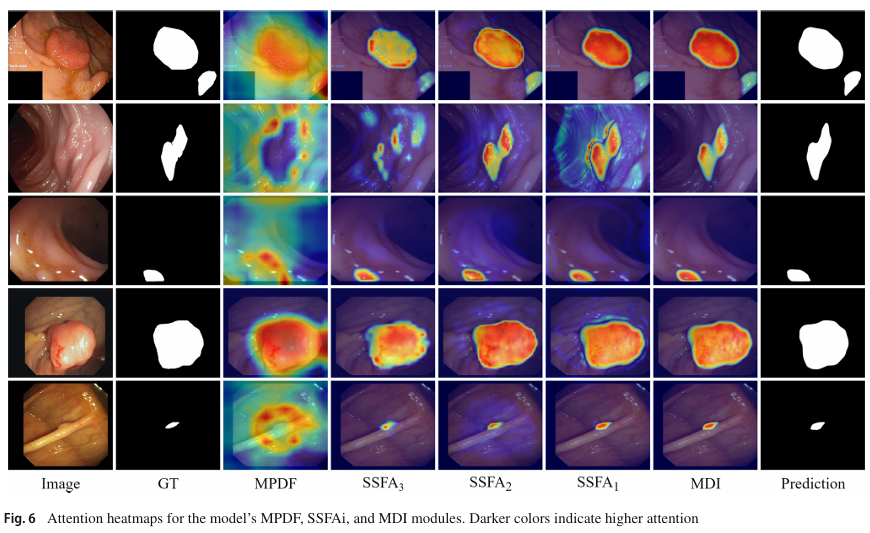
\includegraphics[width=9.06377in,height=5.55286in]{media/image1.png}

\begin{itemize}
\item \textbf{MultiScaleContext}: tests whether multi-scale/global context
helps.

\item \textbf{BSEI}: tests boundary-aware feature enhancement.

\item \textbf{DetailBranch}: tests high-resolution spatial detail recovery.

\item \textbf{GatedDetailFusion}: tests whether adaptive fusion is better
than simple fusion.
\end{itemize}

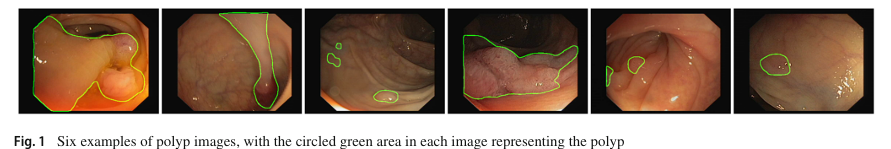
\includegraphics[width=9.28255in,height=1.5523in]{media/image2.png}

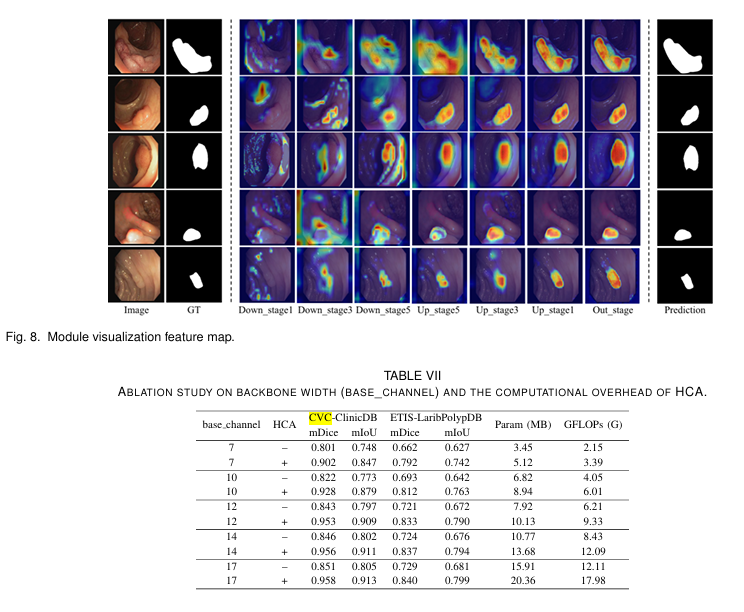
\includegraphics[width=7.75108in,height=6.37589in]{media/image3.png}

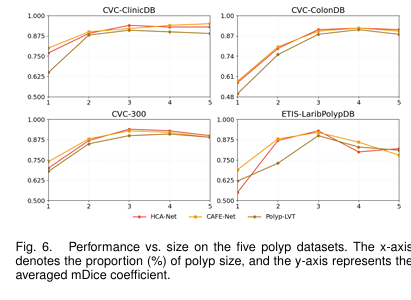
\includegraphics[width=4.28185in,height=3.12544in]{media/image4.png}

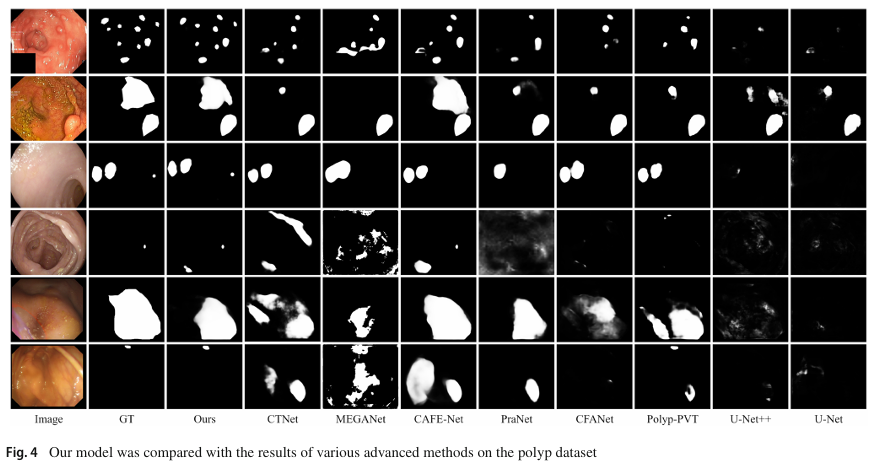
\includegraphics[width=9.0846in,height=4.85484in]{media/image5.png}

\begin{itemize}
\item
  Image(Diagram) of the model with related Modules -\textgreater{} two
  images
\item
  Heatmap of the model in ablation study with 6 samples
\item
  Heatmap of the model for some stages
\item
  Heatmap of the model in comparison with other models
\item
  Table of the ablation study
\end{itemize}

\end{document}
